%%%--------------------------------%%%
%%% Theory
%%%--------------------------------%%%
\newpage
\section{Gamification}
\label{sec:theoryB}

The following chapters aim is to clarify the main theory behind human motivation, gamification and the corresponding patterns and methods. Therefore first of all the term Gamification is defined and explained (chapter \ref{sec:theoryBa}), furthermore there is an introduction to human motivation (chapter \ref{sec:theoryBb}) and motivational patterns (chapter \ref{sec:theoryBc}). Moreover gamification best practices and the gamification process are introduced (chapter \ref{sec:theoryBd}). Finally chances and risks of gamified business applications are discussed (chapter \ref{sec:theoryBe}).


\subsection{Definition Gamification}
\label{sec:theoryBa}

The term gamification is defined by Kumar and Herger as follows:

\begin{fquote}[Gamification {\protect\cite[p. 8]{inproceedings}}]
	Gamification is the application of game design principles and mechanics to
	non-game environments. It attempts to make technology more inviting by encouraging users to engage in desired behaviors and by showing the path to mastery.
	From a business viewpoint, gamification is using people’s innate enjoyment of play.
\end{fquote}

Based on the above definition gamification aims to motivate the user to do something. That is why the next chapter provides a more comprehensive introduction on motivation. \cite[p. 8]{inproceedings}


\subsection{Motivation}
\label{sec:theoryBb}

The game design principles and mechanics which are used in the context of gamification are a specialization of motivational patterns used in Human Computer Interaction. \cite[p. 59]{inproceedings}

Therefore this chapter provides an introduction into the underlying psychology of motivation with the different types of motivation (extrinsic and intrinsic), behavioral psychology and behavioral economics.

\paragraph*{Psychology of motivation}
Human motivation is one of the main areas of psychology. Some questions which arouse are: What motivates humans for doing something? What intentions do they pursue with their doing? Which activities are a pleasure for them? \cite[p. 1]{bierhoffeditorEnzyklopaediePsychologieSoziale2016}

Mainly there are two types of motivation: extrinsic and intrinsic motivation. 
On the one hand intrinsic motivation is based on an internal drive to do something. The human is doing this task for their own. Possible motivational factors are gained autonomy, mastery or freedom. \cite[p. 2, 3, 4]{bierhoffeditorEnzyklopaediePsychologieSoziale2016}, \cite[p. 60, 61]{inproceedings}

Deci describes intrinsic motivation as follows: "One is said to be intrinsically motivated to perform an activity when he receives no apparent rewards except the activity itself." \cite[p. 105]{deciEffectsExternallyMediated1971}

On the other hand extrinsic motivation is based on motivational factors from the outside, such as money, throphys or the comparison with others through (for example with points, levels or leaderboards). \cite[p. 2, 3, 4]{bierhoffeditorEnzyklopaediePsychologieSoziale2016}, \cite[p. 60, 61]{inproceedings}

\label{selfDeterminationTheory}
One theory dealing with the core psychology behind motivation is the self-determination theory by Ryan and Deci. Based on this theory human motivation is depended on the satisfaction of the three psychological basic needs: 
\begin{enumerate}
	\item Autonomy
	%Autonomie
	\item Competence
	%Fähigkeit
	\item Relatedness
	%Zugehörigkeit
\end{enumerate} 
Based on Deci and Ryan whenever humans feel autonomous, competent and related motivation arises. \cite[p. 416-432]{deciTheoriesSocialPsychology2019}
%TODO: Seitenzahl anpassen
%TODO: hier fehlt noch eine etwas granularere Beschreibung und eventuell ein Bsp

TODO einordnen: Flow, Interesse \newline
TODO: Beschreibung \cite[p. 19, 20, 21]{bierhoffeditorEnzyklopaediePsychologieSoziale2016}


\paragraph*{Behavioral psychology}

Behavioral psychology studies the way how humans behave and tries to find underlying patterns which trigger specific behavior. There is a constant stream of inputs (stimuli) to our body. In the field of  behavioral psychology human behavior is seen as a response to these inputs. \cite[p. 10]{lewisIrresistibleAppsMotivational2014}

A concrete application, where behavioral psychology can be observed are learned processes, also known as operant conditioning. Experimental Research in the area of operant conditioning was done by Skinner and his experiments known as Skinner box. For a deeper insight into his experiments, his book "The behavior of organisms" \cite{skinnerBehaviorOrganisms1938} is referred. By rewards for desired behavior and punishment for undesired behavior humans get conditioned for specific desired behaviors. Rewards and punishments are the stimuli causing responses. \cite[p. 11]{lewisIrresistibleAppsMotivational2014}

Moreover the time when rewards are provided, influences how the interaction works.
Based on Lewis \cite[p. 10]{lewisIrresistibleAppsMotivational2014} there are four different strategies:
\begin{enumerate}
	\item Fixed Ratio: After a fixed number of responses rewards are provided (e.g. coffee card: the tenth coffee for free)
	\item Variable Ratio: Reward frequency is not firmly defined, the reward is offered on average after a couple of responses (e.g. gambling machine)
	\item Fixed Interval: Rewards are provided after a fixed period of time (e.g. coffee machine)
	\item Variable Interval: The interval in which rewards are offered is variable (e.g. fishing)
\end{enumerate}

The most response over time is generated by variable ratio strategy. So in case of designing engaging applications, connecting the user with this application one should consider the use of rewards in a variable ratio. \cite[p. 11]{lewisIrresistibleAppsMotivational2014}

So large parts of the gamification principles are based on rewards (e.g. increasing points, levels) and punishments (e.g decreasing points and levels). However the application of these principles should always be done carefully. There is a thought experiment by Schell called "chocofication". First of all there is the fact that chocolate tastes good. Adding chocolate to peanut butter makes it tasting good. But regardless the conclusion that everything tastes good with chocolate is wrong. For example hot dogs with chocolate are a disaster. 
To conclude you can say, that based on the thought experiment chocolate is not the magic bullet for food, alike gamification is not the magic bullet for application design. \cite[p. 12]{lewisIrresistibleAppsMotivational2014}


\paragraph*{Behavioral economics}

Behavioral economics explores, which effects affect economic decisions. In general whenever a resource (e.g. time, money) is reached or lost it is the consequence of a decision. So behavioral economics could also be seen as the theory behind decision making. Moreover in the context of Human Computer Interaction whenever a user interacts with an application 
lots of decisions are made. Engaging application design tries to include aspects of behavioral economics to influence the users decisions to spend more time in the application. 
Human decisions could be rational or irrational. Rational decisions are made to reach a concrete aim such as happiness and can be logically explained. Irrational decisions are not necessarily comprehensible.  Nevertheless irrational decisions can be triggered by external influences. For example people tend to use memberships, even if they doesn't profit (e.g. injured people go to the gym to use the membership).
Referring to the relationship between behavioral economics and application design the application can be designed to trigger the user to made an irrational decision (e.g. spend more time inside the application than needed). \cite[p. 19]{lewisIrresistibleAppsMotivational2014}


Patterns which motivate the user to do something by using the theoretical background of motivation, behavioral psychology and behavioral economics are described in the following chapter \ref{sec:theoryBc}

%====================\newline
%Psychologie (was motiviert allgemein) -> übertragen auf die Mensch-Maschine-Interaktion = Human Computer Interaction (Wie agiert der Mensch mit dem Computer/der Maschine)


\subsection{Motivational Patterns}
\label{sec:theoryBc}

The theoretical concepts above are used in various motivational patterns. In Lewis \cite{lewisIrresistibleAppsMotivational2014} and Kumar and Herger \cite{inproceedings} lots of motivational patterns are described. In the following some patterns which may be relevant for the conception of the risk management application are introduced. For a more comprehensive entry into motivational design patterns please refer to \cite{lewisIrresistibleAppsMotivational2014} and \cite{inproceedings}.

\paragraph*{Gameful Patterns}
\label{GamefulPatterns}
\begin{itemize}
	\item Collection: Collecting and owning virtual items (e.g. Forza Horizon, Pokémon). \cite[p. 4, 35]{lewisIrresistibleAppsMotivational2014}
	\item Specialization—Badge: The user has reached a goal which is now visible through a badge (e.g. Xbox 360). \cite[p. 4, 37]{lewisIrresistibleAppsMotivational2014}
	\item Growth: User owns something which was reached over time (e.g. SimCity). \cite[p. 4, 40]{lewisIrresistibleAppsMotivational2014}
	\item Increased Responsibility: Trust in a user is the underlying basis for getting responsible tasks (e.g. Stack Overflow). \cite[p. 4, 41]{lewisIrresistibleAppsMotivational2014}
	\item Leaderboard: Ranking users based on specific metrics (e.g. Doodle Jump). \cite[p. 4, 44]{lewisIrresistibleAppsMotivational2014}
	\item Score: Based on the reward principle. By performing desired behavior the user normally achieves points, presenting his/her achievement level (e.g. Pac-Man) \cite[p. 4, 46]{lewisIrresistibleAppsMotivational2014}
	\item Challenge: Challenges motivate users by giving them the feeling of reaching something great (e.g. Runkeeper) \cite[p. 77, 78]{inproceedings}
	\item Constraints with urgent optimism: Urgent Optimism combined with deadlines leads to a motivational effect. \cite[p. 78]{inproceedings}
	\item Journey (Onboarding, Scaffolding, Progress): Journey describes the adaptability of the application based on different usage phases. One can think about a specific onboarding process providing an introduction and help regarding the application. The next phase after onboarding is scaffolding. The user is still inexperienced leading to a risk of operating errors. By providing support and constant feedback the bounce rate is minimized. Finally the user is onboarded and knows the main concepts of the application and is able to use them. Nevertheless the constant user engagement is still desirable. It can be implemented with elements clearly showing users their current progress and feedback loops. (e.g. Setup process for LinkedIn) \cite[p. 80, 81, 82]{inproceedings}
\end{itemize}

\paragraph*{Social Patterns}
\begin{itemize}
	\item Activity Stream: Representation of current events as never ending stream of news (e.g. Facebook). \cite[p. 4, 52]{lewisIrresistibleAppsMotivational2014}
	\item Broadcast: Information can be shared between different users (e.g. Facebook, Twitter). \cite[p. 4, 53]{lewisIrresistibleAppsMotivational2014}
	\item Social Feedback/Feedback loops: Users are able to easily feedback something. Furthermore multiple feedback loops are possible (e.g. Facebook).
	\cite[p. 4, 54]{lewisIrresistibleAppsMotivational2014}
\end{itemize}

\paragraph*{Interface Patterns}
\begin{itemize}
	\item Notifications: The user can be alerted by the application when a change occurs (e.g. Android, iOS) 	\cite[p. 5, 70]{lewisIrresistibleAppsMotivational2014}
	\item Praise: Rewards for performing desired behavior (e.g. FarmVille) \cite[p. 5, 72]{lewisIrresistibleAppsMotivational2014}
	\item Predictable Results: The results of an action are clearly predictable for users. (e.g. Google Search always provides search results) \cite[p. 5, 74]{lewisIrresistibleAppsMotivational2014}
	\item State Preservation: The current state of the application is stored at any time, no matter when the application is left (e.g. Google Docs) \cite[p. 5, 75, 76]{lewisIrresistibleAppsMotivational2014}
	\item Undo: The user is able to revert actions (e.g. Google Docs) \cite[p. 5, 79]{lewisIrresistibleAppsMotivational2014}
\end{itemize}

\paragraph*{Information Patterns}
\begin{itemize}
	\item Organization of Information: When information are presented ordered and organized the retrieval afterwords is simpler (e.g. Outlook) \cite[p. 6, 85, 86]{lewisIrresistibleAppsMotivational2014}
	\item Personalization: Based on the individual user preferences the application adapts itself (e.g. Amazon) \cite[p. 6, 87]{lewisIrresistibleAppsMotivational2014}
	\item Reporting: Reporting inappropriate content by users is possible (e.g. Facebook) \cite[p. 6, 90]{lewisIrresistibleAppsMotivational2014}
	\item Search: Huge content is easily searchable (e.g. Google Search) \cite[p. 6, 90, 91]{lewisIrresistibleAppsMotivational2014}
	\item Task Queue: Presents tasks which can be done next by a user trying to keep the user using the application (e.g. Setup process for LinkedIn) \cite[p. 6, 93]{lewisIrresistibleAppsMotivational2014}
\end{itemize}


\subsection{Gamification best practices and process}
\label{sec:theoryBd}

According to \cite[p. 5, 6]{lowdermilkUsercenteredDesignDevelopers2013} and \cite[p. 27, 28]{inproceedings} a well established design philosophy is User Centered Design. The center of the whole design and development of the application is the user. With this approach it gets possible to match the users needs. The developed application is intuitively operable for the user and increases the user's productivity.

In the context of gamification the User Centered Design Process can be adapted to be a Player Centered Design Process.  

Based on \cite[p. 29-32]{inproceedings} it consists of five steps:
\begin{enumerate}
	\item Player \newline
	Firstly it should be clearly defined who is the user, respectively the player. Based on a profound knowledge of the player and his needs the application can be designed. Therefore user/player personas are created, describing different users/player types, interacting with the application. The following user/player persona template is based on \cite[p. 38-45]{inproceedings}:

	\begin{figure}[htbp] 
		\centering
		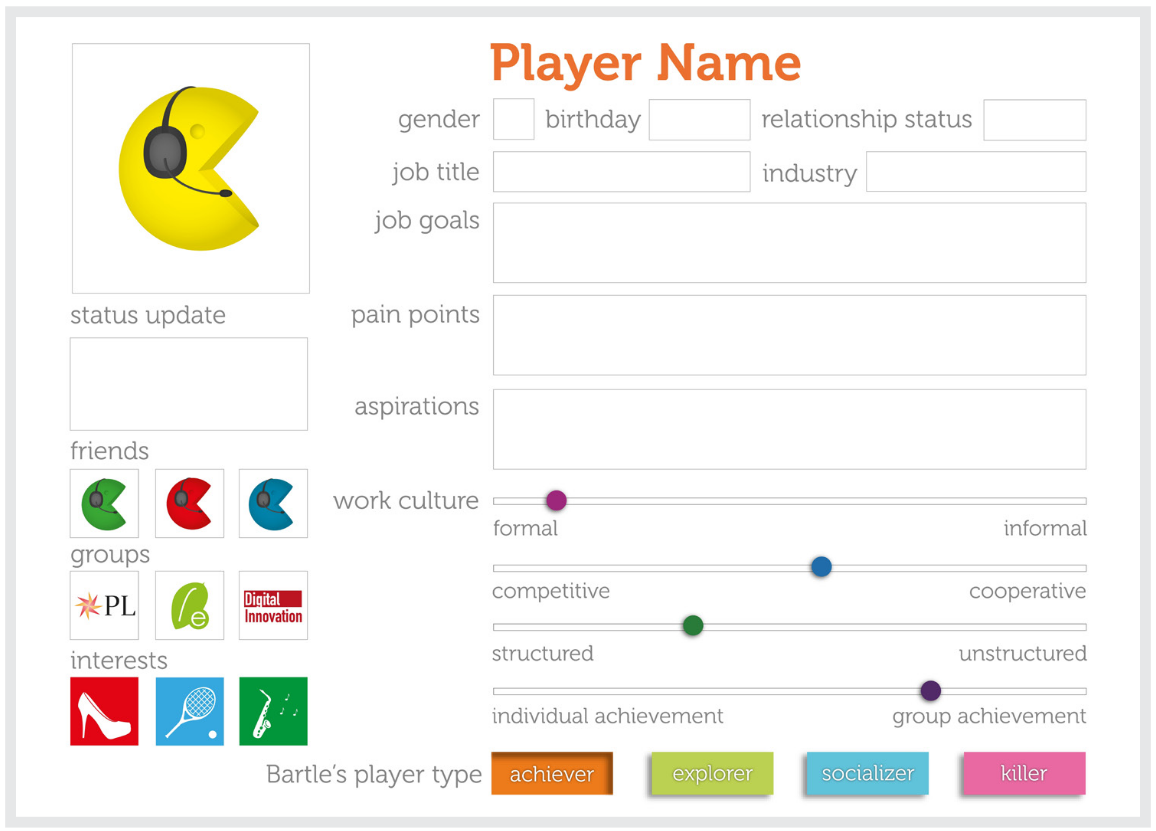
\includegraphics[width=1.0\textwidth]{Content/Theory/PlayerPersona.png}
		\caption{Player Persona Template}
		\cite[p. 46]{inproceedings}
		\label{fig:playerPersonaTemplate}
	\end{figure}

	TODO: formal, informal, ... -> Glossar
	TODO: Bartle Player types beschreiben
	
	\item Mission \newline
	Secondly the main goal of the gamification process identified, the so called mission. Figure \ref{fig:smartMission} represents the S.M.A.R.T Mission process to identify the mission. First of all the current situation is analyzed and the target business outcome is studied. Based on the gained knowledge a mission for the gamification process is set. It should be specific, measurable, actionable, realistic and time-bound. \cite[p. 49-52]{inproceedings}
	
	\begin{figure}[htbp] 
		\centering
		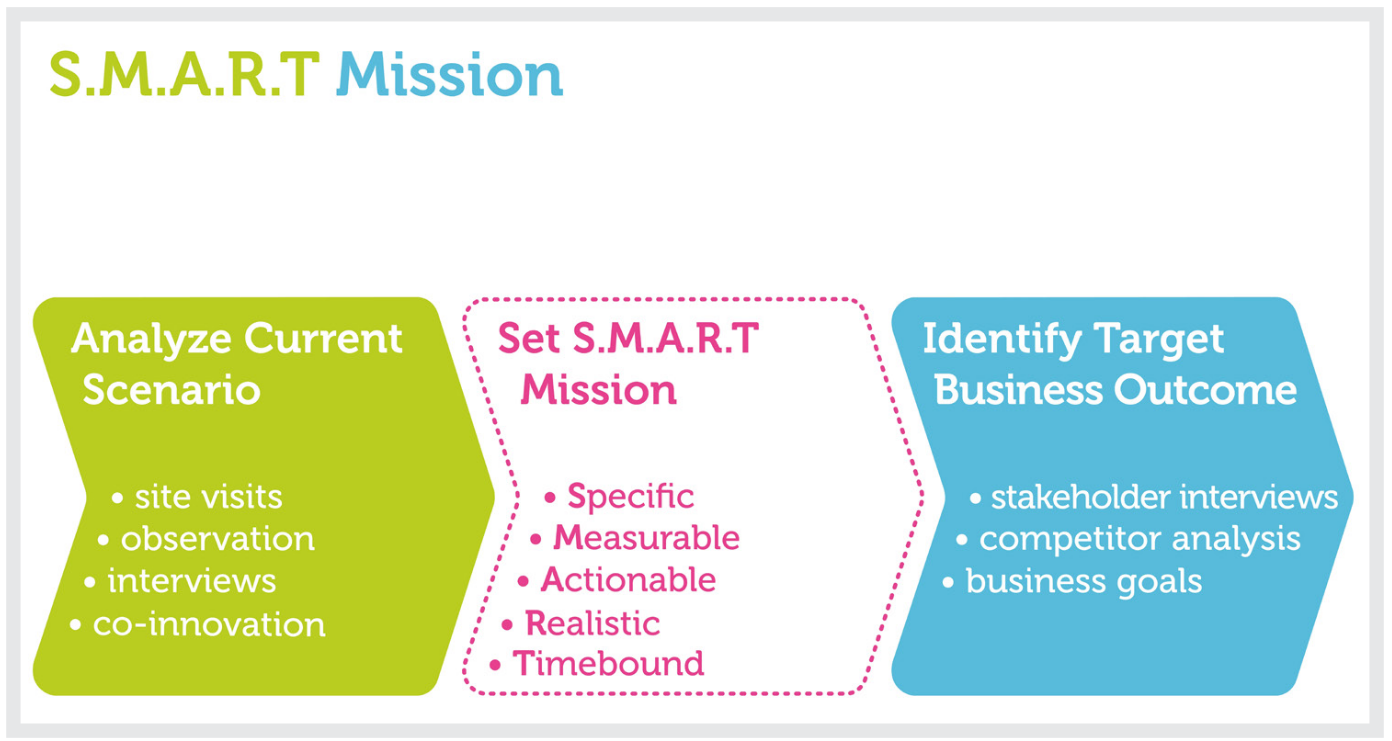
\includegraphics[width=1.0\textwidth]{Content/Theory/SmartMission.png}
		\caption{S.M.A.R.T. Mission}
		\cite[p. 50]{inproceedings}
		\label{fig:smartMission}
	\end{figure}

	\item Human Motivation \newline
	Thirdly a basic knowledge about the theory behind human motivation is needed and is therefore described in chapter \ref{sec:theoryBb}.
	
	\item Game Mechanics \newline
	Game mechanics represent the area of adding concrete gameful patterns to a non game environment. As part of motivational patterns gameful patterns are described in chapter \ref{GamefulPatterns}. While implementing gameful patterns in non game environments one should take into account that adding all patterns to an application normally doesn't reach the resumed aim. Hence the selection of fitting patterns must be adapted to the prescribed context. The main aim behind adding gameful patterns is to build a positive engagement loop centering the user/player. Figure \ref{fig:engagementLoop} shows the four main steps of the engagement loop, starting with a motivating emotion.  \cite[p. 69-71]{inproceedings}
	
	\begin{figure}[htbp] 
		\centering
		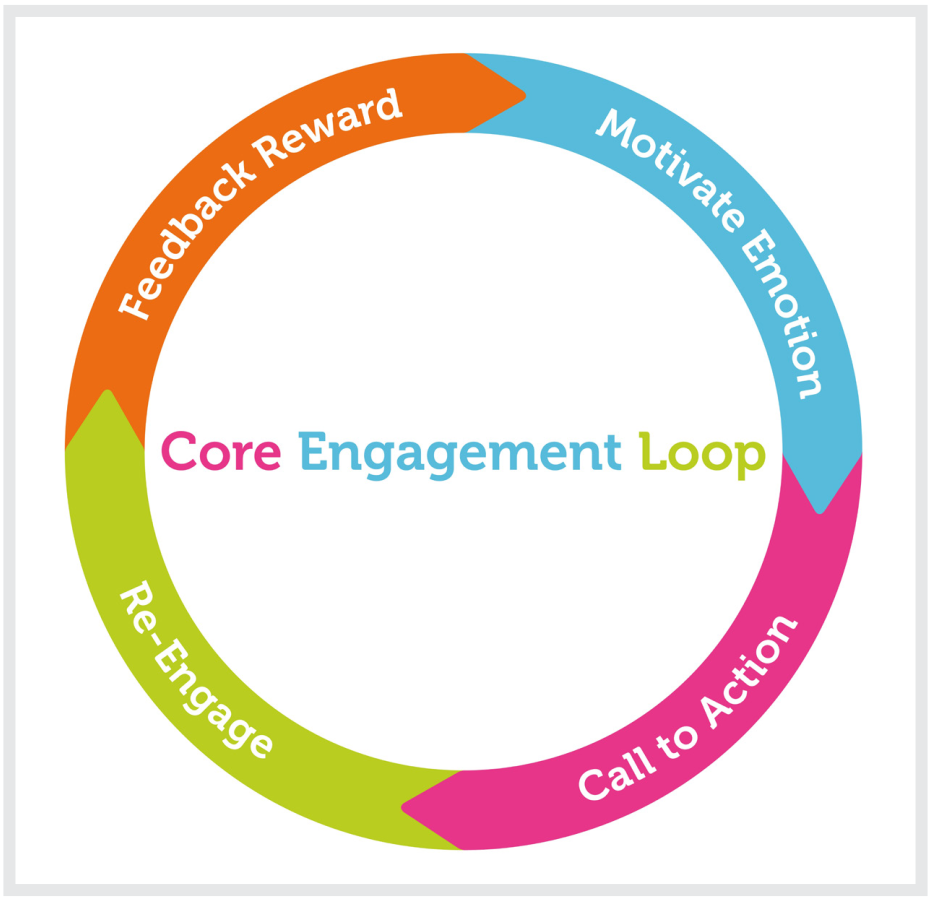
\includegraphics[width=1.0\textwidth]{Content/Theory/EngagementLoop.png}
		\caption{Engagement Loop}
		\cite[p. 88]{inproceedings}
		\label{fig:engagementLoop}
	\end{figure}
	
	\item Manage, Monitor and Measure \newline
	After applying specific game mechanics to an application there are few points left, which should be observed in production. On the one hand the mission should be managed. Based on the S.M.A.R.T. Mission process the identified mission should be checked frequently and if needed adapted. On the other hand the user/player behavior should be monitored and measured to evaluate the effectiveeness of the implemented patterns. This can be done qualitative by surveys and interviews and quantitative by tracking and data evaluation. Based on the acquired knowledge the application can be enhanced in the future.	\cite[p. 92-96]{inproceedings}
\end{enumerate}


\subsection{Chances and risks of Gamification}
\label{sec:theoryBe}

A literature review from Hamari, Koivisto and Sarsa \cite{hamariDoesGamificationWork2014} tries to answer the question if gamification works. Therefore quantitative and qualitative studies on this topic had been analyzed, resulting in the statement that quantitatively there are positive effects of gamification, but the gamification elements are only partly responsible for these effects. The analysis of qualitative studies has resulted in the statement that gamification is more versatile than often assumed. The next arousing question is: What are the reasons for these results and which disruptive factors harm the effectiveness of gamification? Therefore the study's conclusions are analyzed resulting in two aspects \cite[p. 3029, 3030]{hamariDoesGamificationWork2014}:
\begin{enumerate}
	\item Influence of the gamified context: \newline
	On the one hand the context which should be gamified influences the prospects of success.  Hamari, Koivisto and Sarsa name three contextual factors \cite[p. 3029, 3030]{hamariDoesGamificationWork2014}:
	\begin{enumerate}
		\item Social environment: \newline
		In order to form behaviors  one key for success is the voluntariness of doing something. \cite[p. 3030]{hamariDoesGamificationWork2014}
		
		\item Nature of the system: \newline
		Is the system which should be gamified hedonic or utilitarian? Hedonic systems support their users reaching desire and pleasure. \cite[p. 3030]{hamariDoesGamificationWork2014}
		They are based on the philosophical concept of hedonism, which centers the human pursuit of desire and pleasure. Only the steady pursuit can reach intrinsically motivation. TODO: valide Quelle!
		
		On the contrary utilitarian systems are purpose-oriented. The underlying philosophical concept is the utilitarianism. It is based on the principle that an action is morally correct when it maximizes the aggregated overall benefit, that is the sum of the welfare of all concerned. TODO: valide Quelle!
		
		\item Involvement of the user: \newline
		Depending on the application's context there are two types how a user can be involved: cognitive or affective. \cite[p. 3030]{hamariDoesGamificationWork2014} Cognitive involvement describes the user's interest respective an application. When being affectively involved, one evolves specific feelings regarding the application. In the context of business application normally the user's are involved cognitively. \cite{zaichkowskyPersonalInvolvementInventory2013}
	\end{enumerate}

	%Korrumpierungseffekt
	Furthermore the overjustification effect describes the consequences how intrinsically motivated user's change their behavior when extrinsic incentives are added. By adding extrinsic motivation the intrinsic motivation decreases. \cite[p. 9-13]{bierhoffeditorEnzyklopaediePsychologieSoziale2016}
	
	Moreover there is the risk of false incentives. When applying gamification patterns without really thinking about the consequences it can lead to misguided behavior. E.g. when every user who contributes a risk to the project get points, there was a false incentive created, leading to lots of contributed risks, but little attention for the risk management of each risk. \cite[p.69]{inproceedings}
	
	\item User qualities: \newline
	On the other hand the different abilities and qualities of users have a decisive influence on the users behavior while using the application and thus the success of gamification. Each user interacts differently with the application. E.g. positive gamification effects where only measurable inside a specific context or with specific users. \cite[p. 3029, 3030]{hamariDoesGamificationWork2014}
\end{enumerate}


\newpage
